%%%% Paramétrage du TD %%%%
\def\xxactivite{Révisions \ifprof -- Corrigé \else \fi} % \normalsize \vspace{-.4cm}
\def\xxauteur{\textsl{Xavier Pessoles}}


\def\xxnumchapitre{Révision 1 \vspace{.2cm}}
\def\xxchapitre{\hspace{.12cm} Résolution des problèmes de statique -- Statique 2D}
\def\xxonglet{\textsf{Rév -- Stat}}
\def\xxactivite{TD 01}
\def\xxauteur{\textsl{Xavier Pessoles}}

\def\xxpied{%
Documents de TP\\
Étude théorique de la barrière Sympact\xxactivite%
}

\def\xxcompetences{%
\vspace{-.3cm}
\textsl{%
\textbf{Savoirs et compétences :}\\
%\vspace{-.4cm}
%\begin{itemize}[label=\ding{112},font=\color{ocre}] 
%%\item \textit{Res1.C4 : } Correction
% \item \textit{Res1.C4.SF1 : } Proposer la démarche de réglage d’un correcteur proportionnel
%%proportionnel intégral 
%%et à avance de phase
%\item \textit{Con.C2 : } 	Correction d’un système asservi	
%\item \textit{Con.C2.SF1 : } Choisir un type de correcteur adapté
%\end{itemize}
}}

\def\xxauteur{\textsl{Xavier Pessoles}}

\def\xxtitreexo{Documents de TP}
\def\xxsourceexo{\hspace{.2cm} \footnotesize{Étude théorique de la barrière Sympact}}

\def\xxfigures{
%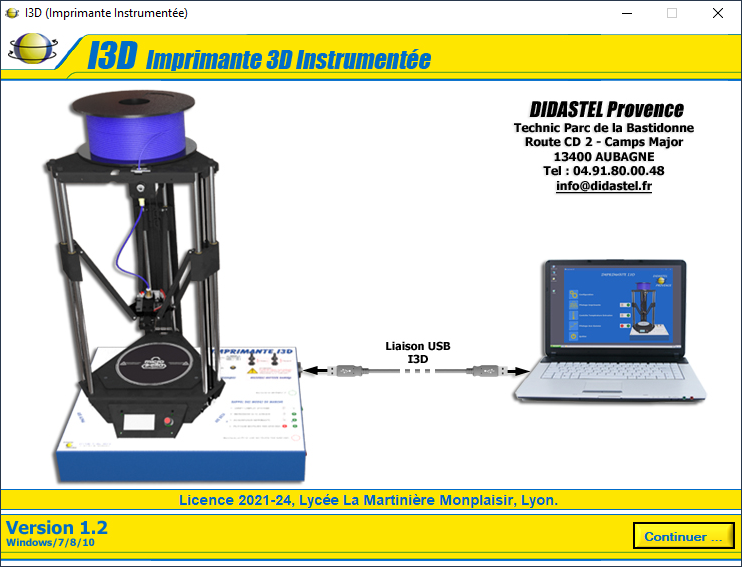
\includegraphics[width=.55\textwidth]{fig_00}
}%figues de la page de garde


\iflivret
\pagestyle{empty}


%%%%%%%% PAGE DE GARDE COURS
\ifcours
\begin{tikzpicture}[remember picture,overlay]
\node at (current page.north west)
{\begin{tikzpicture}[remember picture,overlay]
\node[anchor=north west,inner sep=0pt] at (0,0) {\includegraphics[width=\paperwidth]{\thechapterimage}};
\draw[anchor=west] (-2cm,-8cm) node [line width=2pt,rounded corners=15pt,draw=ocre,fill=white,fill opacity=0.6,inner sep=40pt]{\strut\makebox[22cm]{}};
\draw[anchor=west] (1cm,-8cm) node {\huge\sffamily\bfseries\color{black} %
\begin{minipage}{1cm}
\rotatebox{90}{\LARGE\sffamily\textsc{\color{ocre}\textbf{\xxnumpartie}}}
\end{minipage} \hfill
\begin{minipage}[c]{14cm}
\begin{titrepartie}
\begin{flushright}
\renewcommand{\baselinestretch}{1.1} 
\Large\sffamily\textsc{\textbf{\xxpartie}}
\renewcommand{\baselinestretch}{1} 
\end{flushright}
\end{titrepartie}
\end{minipage} \hfill
\begin{minipage}[c]{3.5cm}
{\large\sffamily\textsc{\textbf{\color{ocre} \discipline}}}
\end{minipage} 
 };
\end{tikzpicture}};
\end{tikzpicture}


\begin{tikzpicture}[overlay]
\node[shape=rectangle, 
      rounded corners = .25 cm,
	  draw= ocre,
	  line width=2pt, 
	  fill = ocre!10,
	  minimum width  = 2.5cm,
	  minimum height = 3cm,] at (18cm,0) {};
\node at (17.7cm,0) {\rotatebox{90}{\textbf{\Large\color{ocre}{\classe}}}};
%{};
\end{tikzpicture}

\vspace{3.5cm}

\begin{tikzpicture}[remember picture,overlay]
\draw[anchor=west] (-2cm,-6cm) node {\huge\sffamily\bfseries\color{black} %
\begin{minipage}{2cm}
\begin{center}
\LARGE\sffamily\textsc{\color{ocre}\textbf{\xxactivite}}
\end{center}
\end{minipage} \hfill
\begin{minipage}[c]{15cm}
\begin{titrechapitre}
\renewcommand{\baselinestretch}{1.1} 
\Large\sffamily\textsc{\textbf{\xxnumchapitre}}

\Large\sffamily\textsc{\textbf{\xxchapitre}}
\vspace{.5cm}

\renewcommand{\baselinestretch}{1} 
\normalsize\normalfont
\xxcompetences
\end{titrechapitre}
\end{minipage}  };
\end{tikzpicture}
\vfill

\begin{flushright}
\begin{minipage}[c]{.3\linewidth}
\begin{center}
\xxfigures
\end{center}
\end{minipage}\hfill
\begin{minipage}[c]{.6\linewidth}
\startcontents
\printcontents{}{1}{}
\end{minipage}
\end{flushright}

\begin{tikzpicture}[remember picture,overlay]
\draw[anchor=west] (4.5cm,-.7cm) node {
\begin{minipage}[c]{.2\linewidth}
\begin{flushright}

\includegraphics[width=2cm]{png/logoCC}
\end{flushright}
\end{minipage}
\begin{minipage}[c]{.2\linewidth}
\textsl{\xxauteur} \\
\textsl{\classe}
\end{minipage}
 };
\end{tikzpicture}
\newpage
\pagestyle{fancy}

\newpage
\pagestyle{fancy}

\else
\fi


%%%%%%%% PAGE DE GARDE TD
\iftd
\begin{tikzpicture}[remember picture,overlay]
\node at (current page.north west)
{\begin{tikzpicture}[remember picture,overlay]
\draw[anchor=west] (-2cm,-3.25cm) node [line width=2pt,rounded corners=15pt,draw=ocre,fill=white,fill opacity=0.6,inner sep=40pt]{\strut\makebox[22cm]{}};
\draw[anchor=west] (1cm,-3.25cm) node {\huge\sffamily\bfseries\color{black} %
\begin{minipage}{1cm}
\rotatebox{90}{\LARGE\sffamily\textsc{\color{ocre}\textbf{\xxnumpartie}}}
\end{minipage} \hfill
\begin{minipage}[c]{13.5cm}
\begin{titrepartie}
\begin{flushright}
\renewcommand{\baselinestretch}{1.1} 
\Large\sffamily\textsc{\textbf{\xxpartie}}
\renewcommand{\baselinestretch}{1} 
\end{flushright}
\end{titrepartie}
\end{minipage} \hfill
\begin{minipage}[c]{3.5cm}
{\large\sffamily\textsc{\textbf{\color{ocre} \discipline}}}
\end{minipage} 
 };
\end{tikzpicture}};
\end{tikzpicture}

%%%%%%%%%% PAGE DE GARDE TD %%%%%%%%%%%%%%%
\begin{tikzpicture}[overlay]
\node[shape=rectangle, 
      rounded corners = .25 cm,
	  draw= ocre,
	  line width=2pt, 
	  fill = ocre!10,
	  minimum width  = 2.5cm,
	  minimum height = 2.5cm,] at (18.5cm,0) {};
\node at (17.7cm,0) {\rotatebox{90}{\textbf{\Large\color{ocre}{\classe}}}};
%{};
\end{tikzpicture}

% PARTIE ET CHAPITRE
\begin{tikzpicture}[remember picture,overlay]
\draw[anchor=west] (-1cm,-2.1cm) node {\large\sffamily\bfseries\color{black} %
\begin{minipage}[c]{15cm}
\begin{flushleft}
\xxnumchapitre \\
\xxchapitre
\end{flushleft}
\end{minipage}  };
\end{tikzpicture}

% Bandeau titre exo
\begin{tikzpicture}[remember picture,overlay]
\draw[anchor=west] (-2cm,-6cm) node {\huge\sffamily\bfseries\color{black} %
\begin{minipage}{5cm}
\begin{center}
\LARGE\sffamily\color{ocre}\textbf{\textsc{\xxactivite}}

\begin{center}
\xxfigures
\end{center}

\end{center}
\end{minipage} \hfill
\begin{minipage}[c]{12cm}
\begin{titrechapitre}
\renewcommand{\baselinestretch}{1.1} 
\large\sffamily\textbf{\textsc{\xxtitreexo}}

\small\sffamily{\textbf{\textit{\color{black!70}\xxsourceexo}}}
\vspace{.5cm}

\renewcommand{\baselinestretch}{1} 
\normalsize\normalfont
\xxcompetences
\end{titrechapitre}
\end{minipage}  };
\end{tikzpicture}

\else
\fi


%%%%%%%% PAGE DE GARDE FICHE
\iffiche
\begin{tikzpicture}[remember picture,overlay]
\node at (current page.north west)
{\begin{tikzpicture}[remember picture,overlay]
\draw[anchor=west] (-2cm,-3.25cm) node [line width=2pt,rounded corners=15pt,draw=ocre,fill=white,fill opacity=0.6,inner sep=40pt]{\strut\makebox[22cm]{}};
\draw[anchor=west] (1cm,-3.25cm) node {\huge\sffamily\bfseries\color{black} %
\begin{minipage}{1cm}
\rotatebox{90}{\LARGE\sffamily\textsc{\color{ocre}\textbf{\xxnumpartie}}}
\end{minipage} \hfill
\begin{minipage}[c]{14cm}
\begin{titrepartie}
\begin{flushright}
\renewcommand{\baselinestretch}{1.1} 
\large\sffamily\textsc{\textbf{\xxpartie} \\} 

\vspace{.2cm}

\normalsize\sffamily\textsc{\textbf{\xxnumchapitre -- \xxchapitre}}
\renewcommand{\baselinestretch}{1} 
\end{flushright}
\end{titrepartie}
\end{minipage} \hfill
\begin{minipage}[c]{3.5cm}
{\large\sffamily\textsc{\textbf{\color{ocre} \discipline}}}
\end{minipage} 
 };
\end{tikzpicture}};
\end{tikzpicture}


\begin{tikzpicture}[overlay]
\node[shape=rectangle, 
      rounded corners = .25 cm,
	  draw= ocre,
	  line width=2pt, 
	  fill = ocre!10,
	  minimum width  = 2.5cm,
	  minimum height = 2.5cm,] at (18.5cm,0) {};
\node at (17.7cm,0) {\rotatebox{90}{\textbf{\large\color{ocre}{\classe}}}};
%{};
\end{tikzpicture}



\else
\fi



\else
\pagestyle{empty}


%%%%%%%% PAGE DE GARDE COURS
\ifcours
\begin{tikzpicture}[remember picture,overlay]
\node at (current page.north west)
{\begin{tikzpicture}[remember picture,overlay]
\node[anchor=north west,inner sep=0pt] at (0,0) {\includegraphics[width=\paperwidth]{\thechapterimage}};
\draw[anchor=west] (-2cm,-8cm) node [line width=2pt,rounded corners=15pt,draw=ocre,fill=white,fill opacity=0.6,inner sep=40pt]{\strut\makebox[22cm]{}};
\draw[anchor=west] (1cm,-8cm) node {\huge\sffamily\bfseries\color{black} %
\begin{minipage}{1cm}
\rotatebox{90}{\LARGE\sffamily\textsc{\color{ocre}\textbf{\xxnumpartie}}}
\end{minipage} \hfill
\begin{minipage}[c]{14cm}
\begin{titrepartie}
\begin{flushright}
\renewcommand{\baselinestretch}{1.1} 
\Large\sffamily\textsc{\textbf{\xxpartie}}
\renewcommand{\baselinestretch}{1} 
\end{flushright}
\end{titrepartie}
\end{minipage} \hfill
\begin{minipage}[c]{3.5cm}
{\large\sffamily\textsc{\textbf{\color{ocre} \discipline}}}
\end{minipage} 
 };
\end{tikzpicture}};
\end{tikzpicture}


\begin{tikzpicture}[overlay]
\node[shape=rectangle, 
      rounded corners = .25 cm,
	  draw= ocre,
	  line width=2pt, 
	  fill = ocre!10,
	  minimum width  = 2.5cm,
	  minimum height = 3cm,] at (18cm,0) {};
\node at (17.7cm,0) {\rotatebox{90}{\textbf{\Large\color{ocre}{\classe}}}};
%{};
\end{tikzpicture}

\vspace{3.5cm}

\begin{tikzpicture}[remember picture,overlay]
\draw[anchor=west] (-2cm,-6cm) node {\huge\sffamily\bfseries\color{black} %
\begin{minipage}{2cm}
\begin{center}
\LARGE\sffamily\textsc{\color{ocre}\textbf{\xxactivite}}
\end{center}
\end{minipage} \hfill
\begin{minipage}[c]{15cm}
\begin{titrechapitre}
\renewcommand{\baselinestretch}{1.1} 
\Large\sffamily\textsc{\textbf{\xxnumchapitre}}

\Large\sffamily\textsc{\textbf{\xxchapitre}}
\vspace{.5cm}

\renewcommand{\baselinestretch}{1} 
\normalsize\normalfont
\xxcompetences
\end{titrechapitre}
\end{minipage}  };
\end{tikzpicture}
\vfill

\begin{flushright}
\begin{minipage}[c]{.3\linewidth}
\begin{center}
\xxfigures
\end{center}
\end{minipage}\hfill
\begin{minipage}[c]{.6\linewidth}
\startcontents
\printcontents{}{1}{}
\end{minipage}
\end{flushright}

\begin{tikzpicture}[remember picture,overlay]
\draw[anchor=west] (4.5cm,-.7cm) node {
\begin{minipage}[c]{.2\linewidth}
\begin{flushright}

\includegraphics[width=2cm]{png/logoCC}
\end{flushright}
\end{minipage}
\begin{minipage}[c]{.2\linewidth}
\textsl{\xxauteur} \\
\textsl{\classe}
\end{minipage}
 };
\end{tikzpicture}
\newpage
\pagestyle{fancy}

\newpage
\pagestyle{fancy}

\else
\fi


%%%%%%%% PAGE DE GARDE TD
\iftd
\begin{tikzpicture}[remember picture,overlay]
\node at (current page.north west)
{\begin{tikzpicture}[remember picture,overlay]
\draw[anchor=west] (-2cm,-3.25cm) node [line width=2pt,rounded corners=15pt,draw=ocre,fill=white,fill opacity=0.6,inner sep=40pt]{\strut\makebox[22cm]{}};
\draw[anchor=west] (1cm,-3.25cm) node {\huge\sffamily\bfseries\color{black} %
\begin{minipage}{1cm}
\rotatebox{90}{\LARGE\sffamily\textsc{\color{ocre}\textbf{\xxnumpartie}}}
\end{minipage} \hfill
\begin{minipage}[c]{13.5cm}
\begin{titrepartie}
\begin{flushright}
\renewcommand{\baselinestretch}{1.1} 
\Large\sffamily\textsc{\textbf{\xxpartie}}
\renewcommand{\baselinestretch}{1} 
\end{flushright}
\end{titrepartie}
\end{minipage} \hfill
\begin{minipage}[c]{3.5cm}
{\large\sffamily\textsc{\textbf{\color{ocre} \discipline}}}
\end{minipage} 
 };
\end{tikzpicture}};
\end{tikzpicture}

%%%%%%%%%% PAGE DE GARDE TD %%%%%%%%%%%%%%%
\begin{tikzpicture}[overlay]
\node[shape=rectangle, 
      rounded corners = .25 cm,
	  draw= ocre,
	  line width=2pt, 
	  fill = ocre!10,
	  minimum width  = 2.5cm,
	  minimum height = 2.5cm,] at (18.5cm,0) {};
\node at (17.7cm,0) {\rotatebox{90}{\textbf{\Large\color{ocre}{\classe}}}};
%{};
\end{tikzpicture}

% PARTIE ET CHAPITRE
\begin{tikzpicture}[remember picture,overlay]
\draw[anchor=west] (-1cm,-2.1cm) node {\large\sffamily\bfseries\color{black} %
\begin{minipage}[c]{15cm}
\begin{flushleft}
\xxnumchapitre \\
\xxchapitre
\end{flushleft}
\end{minipage}  };
\end{tikzpicture}

% Bandeau titre exo
\begin{tikzpicture}[remember picture,overlay]
\draw[anchor=west] (-2cm,-6cm) node {\huge\sffamily\bfseries\color{black} %
\begin{minipage}{5cm}
\begin{center}
\LARGE\sffamily\color{ocre}\textbf{\textsc{\xxactivite}}

\begin{center}
\xxfigures
\end{center}

\end{center}
\end{minipage} \hfill
\begin{minipage}[c]{12cm}
\begin{titrechapitre}
\renewcommand{\baselinestretch}{1.1} 
\large\sffamily\textbf{\textsc{\xxtitreexo}}

\small\sffamily{\textbf{\textit{\color{black!70}\xxsourceexo}}}
\vspace{.5cm}

\renewcommand{\baselinestretch}{1} 
\normalsize\normalfont
\xxcompetences
\end{titrechapitre}
\end{minipage}  };
\end{tikzpicture}

\else
\fi


%%%%%%%% PAGE DE GARDE FICHE
\iffiche
\begin{tikzpicture}[remember picture,overlay]
\node at (current page.north west)
{\begin{tikzpicture}[remember picture,overlay]
\draw[anchor=west] (-2cm,-3.25cm) node [line width=2pt,rounded corners=15pt,draw=ocre,fill=white,fill opacity=0.6,inner sep=40pt]{\strut\makebox[22cm]{}};
\draw[anchor=west] (1cm,-3.25cm) node {\huge\sffamily\bfseries\color{black} %
\begin{minipage}{1cm}
\rotatebox{90}{\LARGE\sffamily\textsc{\color{ocre}\textbf{\xxnumpartie}}}
\end{minipage} \hfill
\begin{minipage}[c]{14cm}
\begin{titrepartie}
\begin{flushright}
\renewcommand{\baselinestretch}{1.1} 
\large\sffamily\textsc{\textbf{\xxpartie} \\} 

\vspace{.2cm}

\normalsize\sffamily\textsc{\textbf{\xxnumchapitre -- \xxchapitre}}
\renewcommand{\baselinestretch}{1} 
\end{flushright}
\end{titrepartie}
\end{minipage} \hfill
\begin{minipage}[c]{3.5cm}
{\large\sffamily\textsc{\textbf{\color{ocre} \discipline}}}
\end{minipage} 
 };
\end{tikzpicture}};
\end{tikzpicture}


\begin{tikzpicture}[overlay]
\node[shape=rectangle, 
      rounded corners = .25 cm,
	  draw= ocre,
	  line width=2pt, 
	  fill = ocre!10,
	  minimum width  = 2.5cm,
	  minimum height = 2.5cm,] at (18.5cm,0) {};
\node at (17.7cm,0) {\rotatebox{90}{\textbf{\large\color{ocre}{\classe}}}};
%{};
\end{tikzpicture}



\else
\fi



\fi
\setlength{\columnseprule}{.1pt}

\pagestyle{fancy}
\thispagestyle{plain}

\vspace{5cm}

\def\columnseprulecolor{\color{ocre}}
\setlength{\columnseprule}{0.4pt} 

\setcounter{exo}{0}

%\ifprof
%%\begin{multicols}{2}
%\else
%\begin{multicols}{2}
%\fi
%%%%%%%%%%%%%%%%%%%%%%%%%%%%%%%%%%%%%%%%%%%%%%%%%%


%\section*{Mise en situation}


\section{Modélisation cinématique de la barrière Sympact}
\subsection{Schéma cinématique}


\begin{center}
 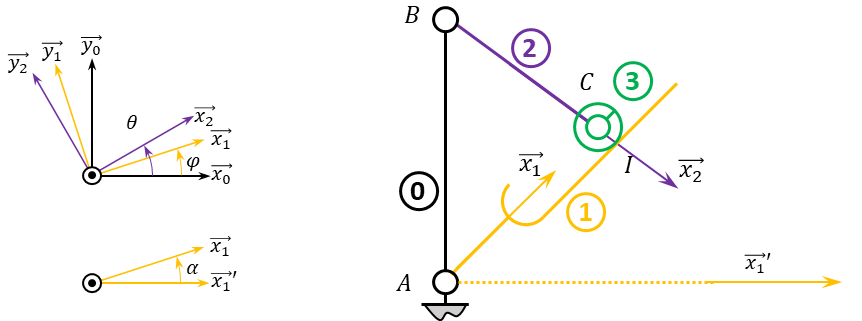
\includegraphics[width=.95\textwidth]{images/fig_01}
\end{center}

On pose $\vect{AB}=H\vect{y_0}$, $\vect{BC}=R\vect{x_2}$ et

$\vect{AC}=\lambda(t)\vect{x_1})$.
\subsection{Détermination de la loi Entrée / Sortie}

La fermeture de chaîne cinématique s'écrit ainsi : $\vect{AB}+\vect{BC}+\vect{CA}=\vect{0}$ soit $H\vect{y_0}+R\vect{x_2}-\lambda(t)\vect{x_1}=\vect{0}$

Projetons cette relation dans le repère $\mathcal{R}_{0}$ :
$H\vect{y_0}+R\left(\cos\theta(t) \vect{x_0}+\sin\theta(t) \vect{y_0}\right) 
-\lambda(t)\left(\cos\varphi(t) \vect{x_0}+\sin\varphi(t) \vect{y_0}\right) 
=\vect{0}$. On a alors :
$\left\{
\begin{array}{l}
R\cos\theta(t) -\lambda(t) \cos\varphi(t) =0 \\
H+R\sin\theta(t) -\lambda(t)\sin\varphi(t) =0
\end{array} 
\right.$


Pour exprimer la loi entrée sortie, il faut déterminer $\varphi$ en fonction de $\theta$.
$\left\{
\begin{array}{l}
R\cos\theta(t) = \lambda(t) \cos\varphi(t)\\
H+R\sin\theta(t) =\lambda(t)\sin\varphi(t)
\end{array} 
\right.$

En faisant le rapport, on a donc $\tan\varphi(t)=\dfrac{H+R\sin\theta(t)}{R\cos\theta(t)}$.



\textbf{Expression analytique de $\lambda$.}
On peut aussi vouloir exprimer $\lambda(t)$ en fonction de $\varphi(t)$ (nécessaire en statique). On a donc :
$\left\{
\begin{array}{l}
R\cos\theta(t) = \lambda(t) \cos\varphi(t)\\
R\sin\theta(t) =\lambda(t)\sin\varphi(t) - H
\end{array} 
\right.$
et $R^2  = \left( \lambda(t) \cos\varphi(t) \right)^2 + \left(\lambda(t)\sin\varphi(t) - H\right)^2$ soit
$R^2  =  \lambda(t)^2+H^2 -2\lambda(t)\sin\varphi(t)  H $.

On résout donc  $ \lambda(t)^2 -2\lambda(t)\sin\varphi(t)  H +H^2 - R^2 = 0$.
$\Delta =  4H^2\sin^2\varphi(t)  -4\left(H^2 - R^2 \right)$ 
 et donc
 
 $\lambda = \dfrac{2\sin\varphi(t) H \pm \sqrt{4H^2\sin^2\varphi(t)  -4\left(H^2 - R^2\right)}}{2}$.
 
 $\lambda = \sin\varphi(t) H \pm \sqrt{H^2\sin^2\varphi(t)  -\left(H^2 - R^2\right)}$.


\subsection{Détermination de la loi en vitesse}
%-u'\rsqcine(1-u²)



\subsection{Tracé des courbes} 
Application numérique : 
%\begin{itemize}
%\item $a = 106,3\; \text{mm}$;
%\item $b = 59 \; \text{mm}$;
%\item $c = 70 \; \text{mm}$;
%\item $d = 80 \; \text{mm}$.
%\end{itemize}

%\begin{center}
%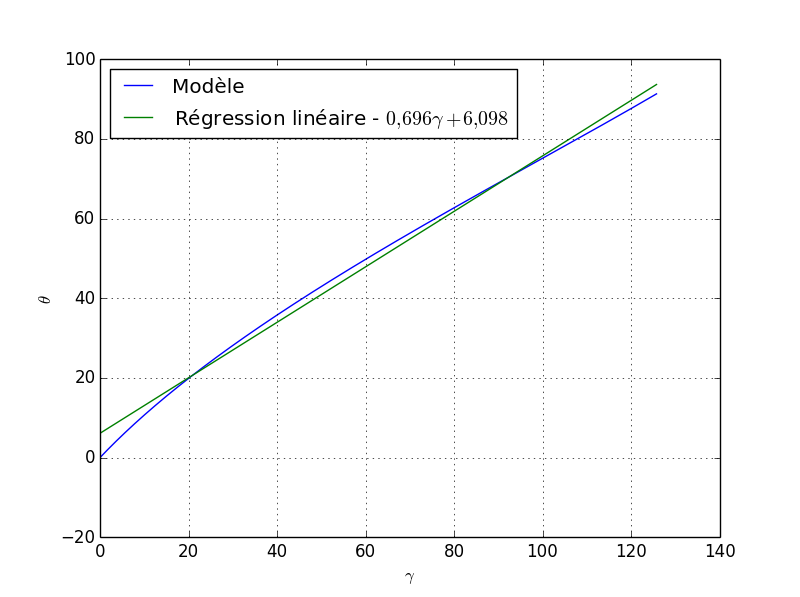
\includegraphics[width=.45\textwidth]{images/LoiTheorique}
%
%\textit{Loi Entrée Sortie -- Position angulaire du bras en fonction de la position du moteur} 
%\end{center}


\section{Détermination du couple moteur en statique}


\begin{center}
 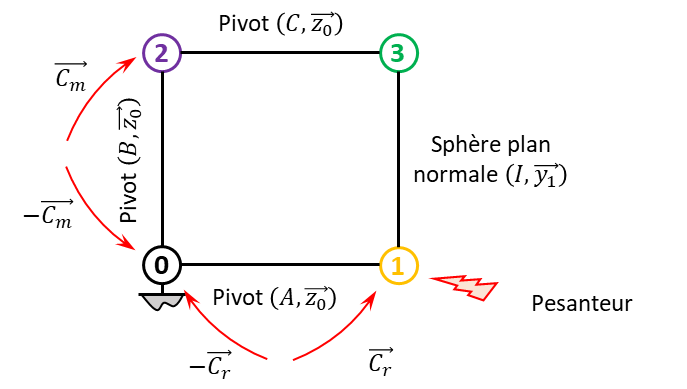
\includegraphics[width=.95\textwidth]{images/fig_02}
\end{center}


\subsection{Isolement du galet 3}
\textbf{On isole le galet (3) soumis à deux glisseurs.}

\textbf{BAME}
\begin{itemize}
\item Pivot entre 2 et 3 : $\torseurstat{T}{2}{3}$.
\item Sphère plan entre 1 et 3 : $\torseurstat{T}{1}{3}$.
\end{itemize}

\textbf{Application du PFS}
D'après le PFS, on a donc :
$\torseurstat{T}{2}{3}+\torseurstat{T}{1}{3}= \{0\}$

soit $\torseurstat{T}{2}{3}=-\torseurstat{T}{1}{3}= \torseurl{F\vect{y_1}}{\vect{0}}{I}$.

\subsection{Isolement de la manivelle 2 + Galet 3}

\textbf{BAME}
\begin{itemize}
\item Pivot entre 0 et 2 : $\torseurstat{T}{0}{2}$.
\item Sphère plan entre 1 et 3 : $\torseurstat{T}{1}{3}= \torseurl{-F\vect{y_1}}{\vect{0}}{I}$ .
\item Moteur entre 0 et 2: $\torseurstat{T}{0}{2}= \torseurl{\vect{0}}{C_m\vect{z_0}}{\forall P}$.
\end{itemize}

\textbf{Application du PFS}

On utilise le théorème du moment statique en $B$ en projection sur l'axe $\vect{z}$.

Déplacement de  $\torseurstat{T}{3}{2}$ en $B$.

On a $\vectm{B}{3}{2}\cdot\vect{z_0}$ 
$=\left(\vectm{I}{3}{2}+\vect{BI}\wedge\vectf{3}{2}\right)\vect{z_0}$

$=\left(\left(\vect{BC}+\vect{CI}\right)\wedge\vectf{3}{2}\right)\vect{z_0}$

$=\left(\left(R\vect{x_2}-r\vect{y_1}\right)\wedge\left(-F\vect{y_1}\right)\right)\vect{z_0}$
$=-rF\left(\vect{x_2}\wedge\vect{y_1}\right)\vect{z_0}$
$=-rF\left(\vect{y_1}\wedge\vect{z_0}\right)\cdot\vect{x_2}$
$=-rF\vect{x_1}\cdot\vect{x_2}$
$=-rF\cos\left( \theta-\varphi\right)$

Le TMS en $B$ s'écrit donc sous la forme 
$C_m=rF\sin\left( \theta-\varphi\right)$


\subsection{Isolement de la barrière 1}

\textbf{BAME}
\begin{itemize}
\item Pivot entre 0 et 1 : $\torseurstat{T}{0}{1}$.
\item Sphère plan entre 1 et 2 : $\torseurstat{T}{3}{2}= \torseurl{-F\vect{y_1}}{\vect{0}}{I}$ .
\item Ressort entre 0 et 1: $\torseurstat{T}{0}{1}= \torseurl{\vect{0}}{C_r\vect{z_0}}{\forall P}$.
\item Pesanteur sur 1: $\torseurstat{T}{\text{pes}}{1}= \torseurl{-Mg\vect{y_0}}{0}{G}$ avec $G$ tel que $\vect{AG}=\mu\vect{x_{1}'}$
\end{itemize}

\textbf{Application du PFS}

On utilise le théorème du moment statique en $A$ en projection sur l'axe $\vect{z}$.

\begin{itemize}
\item Déplacement de  $\torseurstat{T}{3}{2}$ en $A$.

On a $\vectm{A}{3}{2}\cdot\vect{z_0} =\left(\vectm{I}{3}{2}+\vect{AI}\wedge\vectf{3}{2}\right)\vect{z_0}$

$=\left(\left(\vect{AC}+\vect{CI}\right)\wedge\vectf{3}{2}\right)\vect{z_0}$
$=\left(\left(\lambda \vect{x_1}-r\vect{y_1}\right)\wedge\left(-F\vect{y_1}\right)\right)\vect{z_0}$
$=\left(\lambda \vect{x_1}\wedge\left(-F\vect{y_1}\right)\right)\vect{z_0}$
$=-\lambda F$

\item Déplacement de  $\torseurstat{T}{\text{pes}}{1}$ en $A$.
On a $\vectm{A}{\text{pes}}{1}\cdot\vect{z_0} =\left(\vect{AG}\wedge \left(-Mg\vect{y_0}\right)\right)\vect{z_0}$
$=\left(\mu \vect{x_1'}\wedge \left(-Mg\vect{y_0}\right)\right)\vect{z_0}$
$=-Mg \mu \left(\vect{y_0} \wedge \vect{z_0}\right)\vect{x_1'}$
$=-Mg \mu \vect{x_0}\cdot \vect{x_1'}$
$=-Mg \mu \cos\left( \varphi - \alpha \right)$
\end{itemize}

Le TMS en $B$ s'écrit donc sous la forme 
$-\lambda F + C_r-Mg \mu \cos\left( \varphi - \alpha \right) = 0$.

\subsection{Résolution}

On a :
$\left\{
\begin{array}{l}
C_m=rF\sin\left( \theta-\varphi\right) \\
-\lambda F + C_r-Mg \mu \cos\left( \varphi - \alpha \right) = 0 \Leftrightarrow  F=  \dfrac{C_r-Mg \mu \cos\left( \varphi - \alpha \right)}{\lambda} 
\end{array}
\right.
$

On a donc $C_m=r\sin\left( \theta-\varphi\right) \dfrac{C_r-Mg \mu \cos\left( \varphi - \alpha \right)}{\lambda} $.

\subsection{Expression de $C_r$}
La raideur du ressort est de 100\degres pour \SI{40}{Nm} soit $\dfrac{180\times 40}{100 \pi}$ Nm par radian soit \SI{23}{Nm.rad^{-1}} .

De plus, 
$C_r (\varphi) = k\varphi + C_0$
avec  

$\left\{
\begin{array}{l}
C_r\left(\dfrac{3\pi}{4}\right) = 0 =  k\dfrac{3\pi}{4}+ C_0 \\
C_r\left(\dfrac{\pi}{4}\right) =23 \dfrac{\pi}{2}=  k\dfrac{\pi}{4}+ C_0 
\end{array}
\right.$
$ \Leftrightarrow \left\{
\begin{array}{l}
C_0 = - k\dfrac{3\pi}{4}  \\
23 \dfrac{\pi}{2}=  k\dfrac{\pi}{4}- k\dfrac{3\pi}{4} 
\end{array}
\right.$
$ \Leftrightarrow \left\{
\begin{array}{l}
C_0 = 23 \dfrac{3\pi}{4}  \\
k  = -23
\end{array}
\right.$

Au final, $C_r (\varphi) =-23\varphi + 23 \dfrac{3\pi}{4}$.
.


%180° >> pi 
%100° >> 100 pi /180
%100 pi /180 >> 40 N.m
%1 rad >> (40*180)/(100 pi )
\begin{thebibliography}{2}
\bibitem{xx}{xx}
\end{thebibliography}
\end{document}





